\documentclass{beamer}
\usepackage{ctex}
\usepackage[T1]{fontenc}

% other packages
\usepackage{latexsym,amsmath,xcolor,multicol,booktabs,calligra}
\usepackage{graphicx,pstricks,listings,stackengine}
\usepackage{amsthm, amssymb, appendix, bm, mathrsfs}
\usepackage{enumerate}
\usepackage{float}
\usepackage{booktabs}
\usepackage{multirow}
\usepackage{array} 
\usepackage{caption}
\usepackage{subcaption}
\usepackage{geometry}
%\usepackage{algorithm}
%\usepackage{algpseudocode}
\usepackage{hyperref}
\usepackage[linesnumbered,algoruled,boxed,lined]{algorithm2e}%环境
\resetcounteronoverlays{algocf}%加上这条命令阻止算法编号累加
\newcommand{\supcite}[1]{\textsuperscript{\cite{#1}}}
\author{王一鑫}
\title{基于张量分解的神经影像分类模型}
\subtitle{多元统计分析期末汇报}
\institute{兰州大学萃英学院}
\date{\today}
\usepackage{Lanzhou}

% defs
\def\cmd#1{\texttt{\color{red}\footnotesize $\backslash$#1}}
\def\env#1{\texttt{\color{blue}\footnotesize #1}}
\definecolor{deepblue}{rgb}{0,0,0.5}
\definecolor{deepred}{rgb}{0.6,0,0}
\definecolor{deepgreen}{rgb}{0,0.5,0}
\definecolor{halfgray}{gray}{0.55}

\lstset{
	basicstyle=\ttfamily\small,
	keywordstyle=\bfseries\color{deepblue},
	emphstyle=\ttfamily\color{deepred},    
	stringstyle=\color{deepgreen},
	numbers=left,
	numberstyle=\small\color{halfgray},
	rulesepcolor=\color{red!20!green!20!blue!20},
	frame=shadowbox,
}

\begin{document}
	
	\kaishu
	\begin{frame}
		\titlepage
		\begin{figure}[htpb]
			\begin{center}
				\includegraphics[width=0.2\linewidth]{pic/Lanzhou_University_logo.eps}
			\end{center}
		\end{figure}
	\end{frame}
	
	\begin{frame}
		\tableofcontents[sectionstyle=show,subsectionstyle=show/shaded/hide,subsubsectionstyle=show/shaded/hide]
	\end{frame}
	
	\section{引言}
	\begin{frame}{全文概要}
		\begin{itemize}[<+->]
			\item 张量又称多维数组,是矩阵的高维推广。与传统的矩阵(二维数据)不同,张量能够处理更高维度的数据,因此它是多维数据表示的理想工具。
			\item 随着计算能力的突破性进展,张量方法在医学影像分析这类跨学科领域的应用日益扩展。
			\item 在本研究中,我们提出了一种基于高维神经成像数据的贝叶斯张量分类方法。所提出的方法将贝叶斯张量回归应用到了分类问题上。张量结构特别适用于神经成像数据,因为它尊重空间信息,同时通过 PARAFAC 分解进行有效降维。我们实施了两种数据增强方案,通过模拟和数据应用证明了所提方法的优越性。
		\end{itemize}
	\end{frame}
	
	\section{建模方法}
	\subsection{张量及其分解}
	\begin{frame}{张量的概念}
		\begin{exampleblock}{张量}
			张量是一个多维数组,$d$阶张量是一个具有$d$个维度的数组,表示为:
			\[
			\mathcal{X} \in \mathbb{R}^{n_1 \times n_2 \times \cdots \times n_d}
			\]
		\end{exampleblock}
			\begin{figure}[h]
				\small
				\centering
				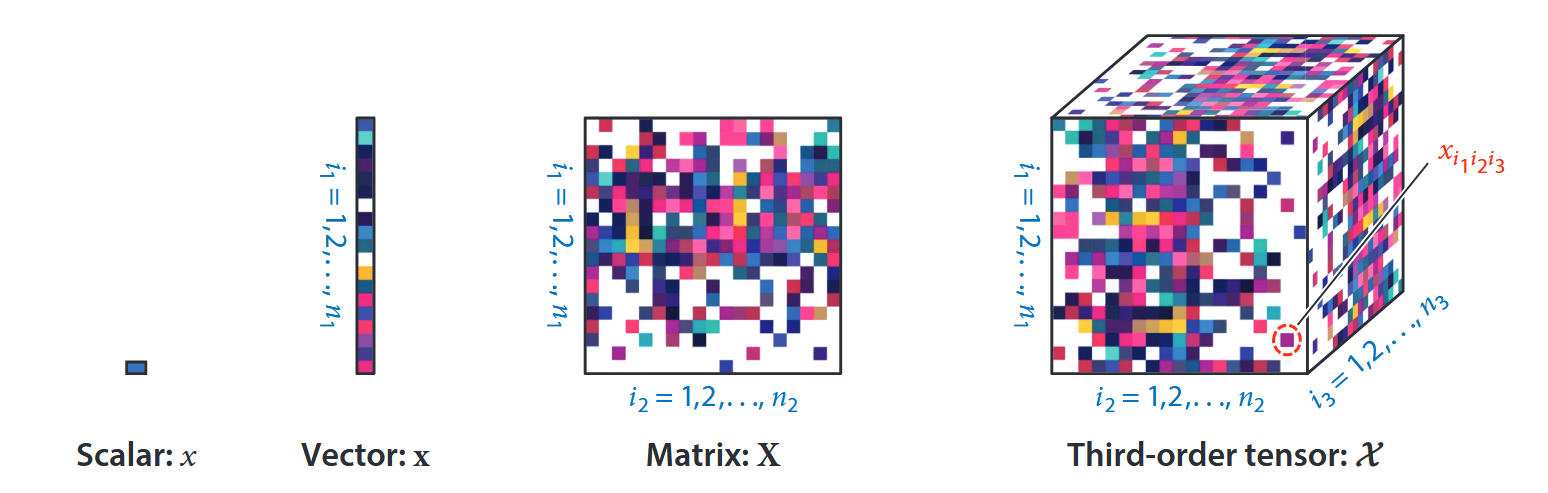
\includegraphics[width=0.8\columnwidth]{../Figure/Example of Tensors.png}
				\caption{标量,向量,矩阵和三阶张量\supcite{a}}
				\label{Fig:Example of Tensors}
			\end{figure}
	\end{frame}
	
	\begin{frame}{Tucker分解}
		\begin{itemize}[<+->]
			\item 张量分解是一种将高维张量分解为若干低维因子组合的技巧,其中一种为Tucker分解,它是张量的高阶主成分分析(PCA),将张量分解为核心张量与各模式因子矩阵的乘积。
			\item 具体地,给定一个张量$\mathcal{X} \in \mathbb{R}^{n_1 \times n_2 \times \cdots \times n_d}$,Tucker分解表示为:
			\begin{exampleblock}{Tucker分解}
				\begin{equation}
					\mathcal{X} \approx \mathcal{C} \times_1 Q^1 \times_2 Q^2 \cdots \times_d Q^d = \sum_{j_1=1}^{m_1} \sum_{j_2=1}^{m_2} \cdots \sum_{j_d=1}^{m_d} c_{j_1 j_2 \dots j_d} 
					\, \mathbf{q}^{1}_{j_1} \circ \mathbf{q}^{2}_{j_2} \circ \cdots \circ \mathbf{q}^{d}_{j_d} \label{Equation:Tucker}
				\end{equation}
			\end{exampleblock}
			\item 其中,$\mathcal{C}\in \mathbb{R}^{m_1 \times m_2 \times \cdots \times m_d}$是核心张量,$Q^{k} \in \mathbb{R}^{n_k \times m_k}$是因子矩阵.
		\end{itemize}
	\end{frame}
	
	\begin{frame}{Tucker分解示意图}
		\begin{figure}
			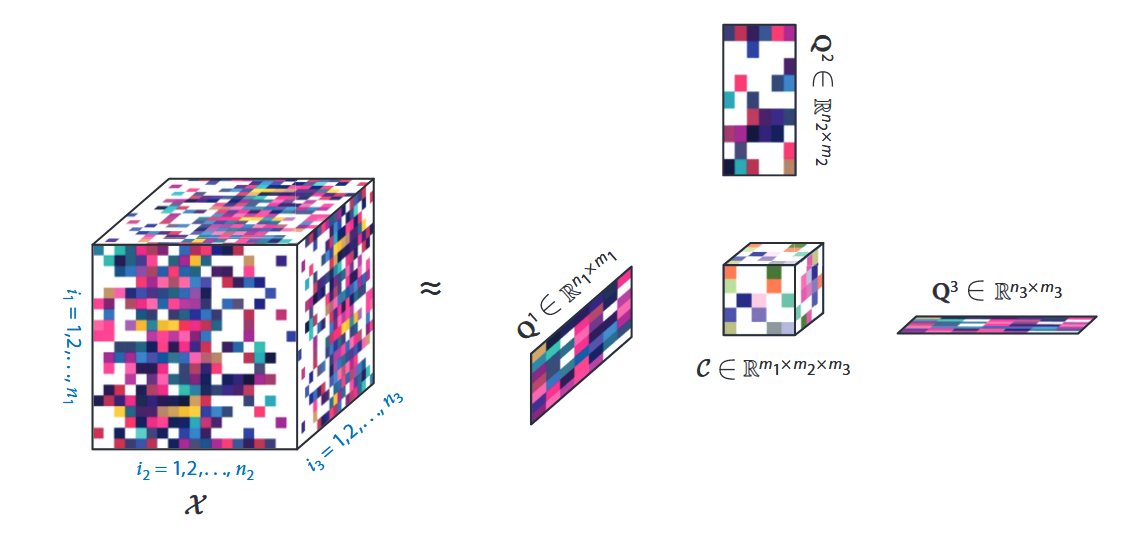
\includegraphics[width=0.8\columnwidth]{../Figure/Tucker.png}
			\caption{Tucker分解示意图\supcite{a}}
		\end{figure}
	\end{frame}
	
	\begin{frame}{PARAFAC分解}
		\begin{itemize}[<+->]
			\item 特别地,当$m_{1} =m_{2} = \cdots =m_{d} = R$,且核心张量限制为对角型时被称为PARAFAC分解. 它将张量近似为一组秩为1的张量的和。具体而言,给定一个张量$\mathcal{X} \in \mathbb{R}^{n_1 \times n_2 \times \cdots \times n_d}$,其分解形式为:
			\begin{exampleblock}{PARAFAC分解}
				\begin{equation}
					\mathcal{X} \approx \sum_{r=1}^{R} \bm{\beta}_1^{(r)} \circ \bm{\beta}_2^{(r)} \circ \cdots \circ \bm{\beta}_d^{(r)}
				\end{equation}
			\end{exampleblock}
			\item 其中$\bm{\beta}_{1},\cdots,\bm{\beta}_{d}$是长度为$p_{1},\cdots,p_{d}$的向量. PARAFAC分解将系数$p_{1}\times\cdots\times p_{d}$降低至$R(p_{1} + p_{2} +\cdots +p_{d})$,提供了有效的降维.
		\end{itemize}
	\end{frame}
	
	\begin{frame}{PARAFAC分解图示}
		\begin{figure}
			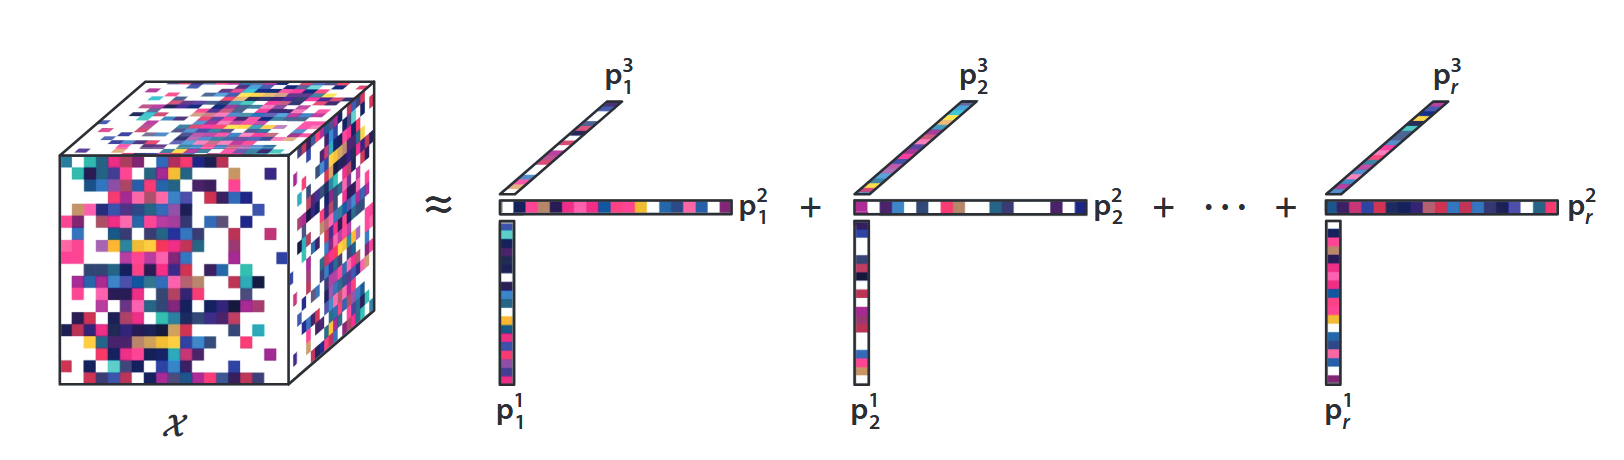
\includegraphics[width=0.8\columnwidth]{../Figure/PARAFAC.png}
			\caption{PARAFAC分解示意图\supcite{a}}
		\end{figure}
	\end{frame}
	\subsection{基于不同损失函数的分类模型}
	\begin{frame}{损失函数}
		\begin{itemize}[<+->]
			\item 损失函数就像是我们用来衡量“错误”的工具。在机器学习中,我们通过这个工具来评判模型训练性能。
			\item 贝叶斯方法中,损失函数转化为不同类型的似然(likelihood)。 通过损失函数结合模型参数的先验假设和真实观测值来更新参数. 通过这种方式,我们可以得到对模型参数的更好估计。
			\item 我们使用了两种常用的损失函数,分别是以支持向量机为代表的铰链损失(hinge loss)和逻辑回归损失(logistic regression loss)。
		\end{itemize}
	\end{frame}
	
	\begin{frame}{Hinge Loss}
		\begin{exampleblock}{Hinge Loss}
			\begin{equation}
				\mathcal{L}(y|\bm{\beta}) = \frac{1}{\sigma^2} \text{max}(1 - y f(\mathbf{x}; \bm{\beta}), 0) + R
			\end{equation}
		\end{exampleblock}
		这里的$y\in\{-1,1\}$是二元输出,$f(\cdot)$是协变量$\mathbf{x}$的线性或非线性函数,$\bm{\beta}$是需要从数据中估计的参数,$\sigma^{2}$是调整参数。
		\begin{figure}
			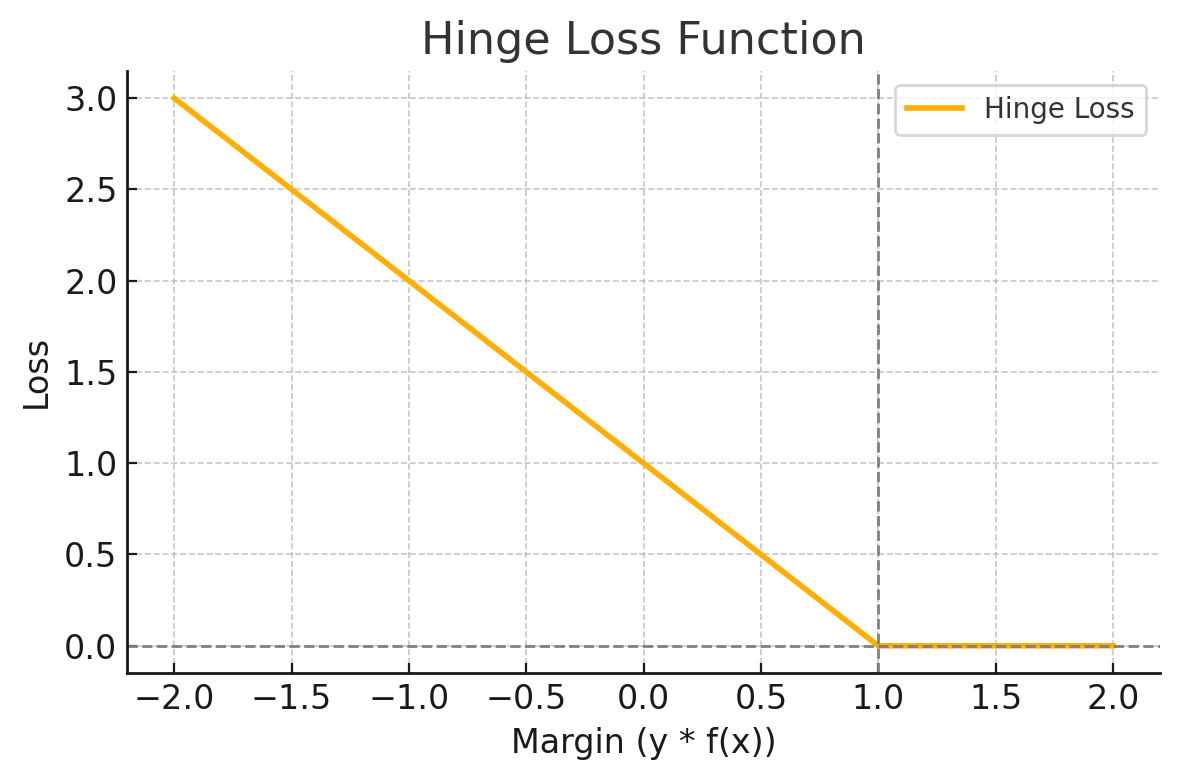
\includegraphics[width=0.4\columnwidth]{../Figure/Hinge Loss.png}
			\caption{SVM的铰链损失}
		\end{figure}
	\end{frame}
	\begin{frame}{伪似然(pseudo-likelihood)方法}
		\begin{itemize}[<+->]
			\item SVM并没有明确的似然函数,不能直接在贝叶斯框架下建模。针对该问题,Polson 和 Scott提出了一种伪似然(pseudo-likelihood)的方法\supcite{c}。
			\item 具体而言,伪似然可以被表示为一种带有潜在变量$\rho$的位置-尺度混合正态分布(location-scale mixture of normals),这种表示法可以为后验推断提供高效的吉布斯采样器。
			\begin{exampleblock}{伪似然方法}
				\begin{align}
					L &= \prod_{i=1}^{n} L_{i}(y_{i}|\mathbf{x}_{i}, \bm{\beta}, \sigma^{2}) \notag 
					= \prod_{i=1}^{n} \left\{ \dfrac{1}{\sigma^{2}} \exp\{-\dfrac{2}{\sigma^{2}} \max\left(1 - y_{i} f(\mathbf{x}; \bm{\beta}), 0 \right)\} \right\}\notag \\
					&= \int_{0}^{\infty}\prod_{i=1}^{n}\dfrac{1}{\sigma\sqrt{2\pi\rho_{i}}}\exp(-\dfrac{(1+\rho_{i} - y_{i}f(\mathbf{x};\bm{\beta}))^{2}}{2\rho_{i}\sigma^{2}})\text{d}\rho_{i}
					\label{Equation:pseudo-likelihood}
				\end{align}
			\end{exampleblock}
		\end{itemize}
	\end{frame}
	\begin{frame}{Logistic Loss}
		\begin{exampleblock}{Logistic Loss}
			\begin{equation}
				\mathcal{L}(y=1|\bm{\beta}) = \frac{\exp\{f(\mathbf{x}; \bm{\beta})\}}{1 + \exp\{f(\mathbf{x}; \bm{\beta})\}}
			\end{equation}
		\end{exampleblock}
		其中,$f(\mathbf{x};\bm{\beta})$代表协变量对逻辑损失的贡献, $\bm{\beta}$为待估参数。
		\begin{figure}
			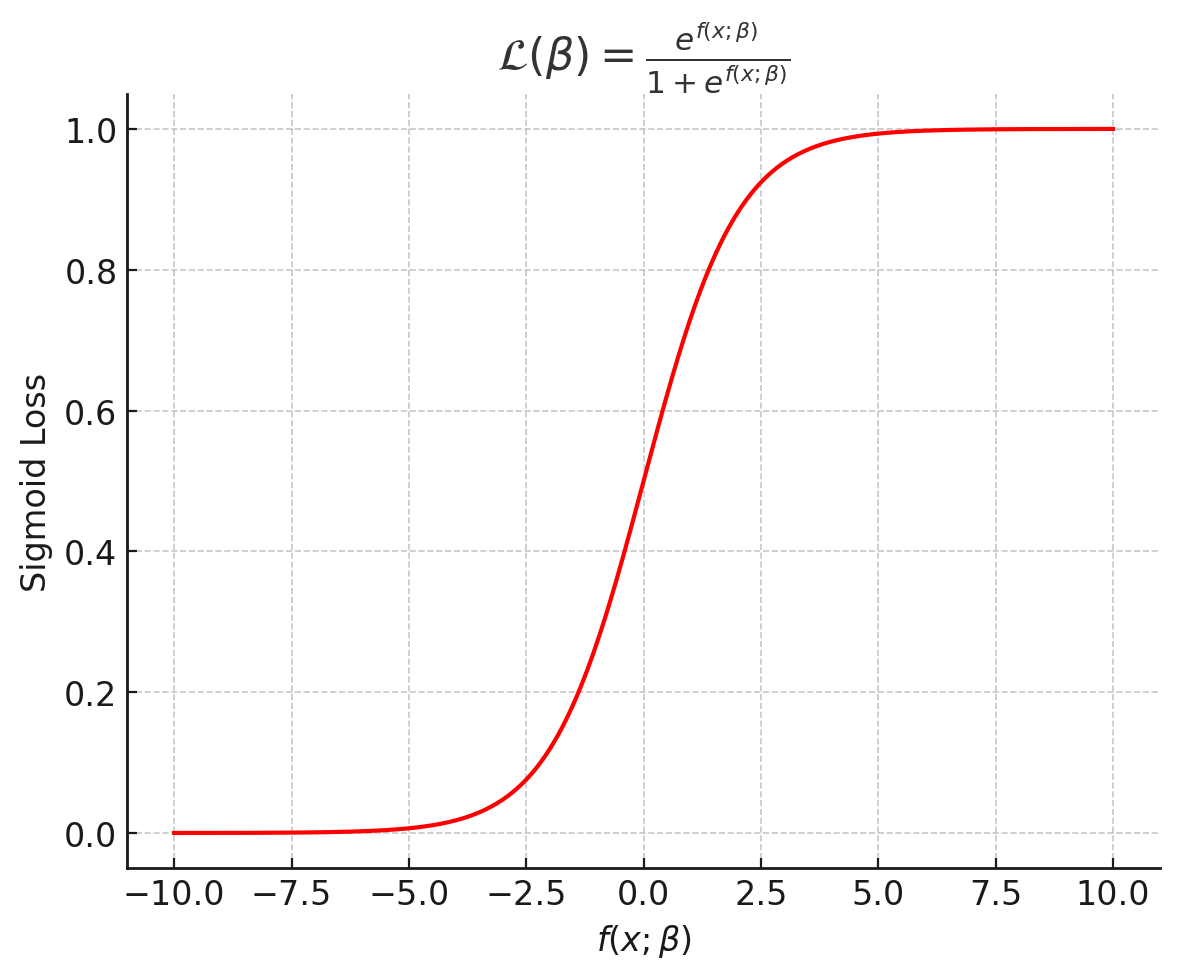
\includegraphics[width=0.4\columnwidth]{../Figure/Logistic Loss.png}
			\caption{逻辑回归损失函数}
		\end{figure}
	\end{frame}
	\begin{frame}{Polya-Gamma潜变量}
		\begin{itemize}[<+->]
			\item 在贝叶斯框架中,逻辑回归的似然函数在分析上并不方便处理,这使得直接从后验分布中采样变得困难。针对此问题,我们通常使用 Polya-Gamma 潜变量来实现\supcite{d}。
			\begin{exampleblock}{Polya-Gamma分布}
				若随机变量$X$有如下形式
				\begin{equation}
					X \overset{D}{=} \dfrac{1}{2\pi^{2}}\sum_{k=1}^{\infty}\dfrac{g_{k}}{(k-1/2)^{2} + c^{2}/(4\pi^{2})
					}
					\label{PG}
				\end{equation}
				则称$X$服从参数为$b>0$, $c\in\mathbb{R}$的Polya-Gamma分布,记作$X~PG(b,c)$. 其中$g_{k}$服从Gamma分布$Ga(b,1)$,相互独立。$\overset{D}{=}$表示在分布意义下相等。
			\end{exampleblock}
		\end{itemize}
	\end{frame}
	\begin{frame}{Polya-Gamma潜变量}
		\begin{itemize}[<+->]
			\item 通过引入 Polya-Gamma 潜在变量可以将对数优势比参数化的二项式似然表示为关于 Polya-Gamma 分布的高斯混合\supcite{d}。
			逻辑损失函数可以通过对潜在的 Polya-Gamma 变量进行边缘化处理而得到,其关系如下所示:
			\begin{exampleblock}{损失函数}
				\begin{equation}
					\frac{(e^{f(\cdot)})^y}{(1 + e^{f(\cdot)})^b} = 2^{-b} e^{\kappa \psi} \int_0^\infty e^{-\omega \psi^2 / 2} p(\omega) \, d\omega,
					\quad b > 0, \quad \kappa = y - \frac{b}{2}
				\end{equation}
			\end{exampleblock}
			\item 其中 \( \omega \sim \text{PG}(b, 0) \),\( p(\omega) \) 表示 Polya-Gamma 分布的密度函数。
		\end{itemize}
	\end{frame}
	\begin{frame}{Polya-Gamma潜变量}
		在该等式基础上,完整的数据增强似然函数为
		\begin{equation}
			L = \prod_{i=1}^n \frac{(e^{f_i})^{y_i}}{1 + e^{f_i}} 
			= \prod_{i=1}^n 2^{-1} e^{\kappa_i \psi_i} \int_0^\infty e^{-\omega_i f_i^2 / 2} p(\omega_i) \, d\omega_i
		\end{equation}
		
		其中$\kappa_i = y_i - \frac{1}{2}$, $b = 1$, $\omega_i \sim \text{PG}(1, 0)$。
	\end{frame}
	\subsection{先验估计}
	\begin{frame}{先验估计}
		\begin{itemize}
			\begin{exampleblock}{线性预测模型}
				\begin{equation}
					f_{i} = \langle \mathbf{X}_{i}, \bm{B}\rangle + \mathbf{z}_{i}^{\prime}\bm{\gamma}
				\end{equation}
			\end{exampleblock}
			\item 这里的 \( \mathbf{X}_i \) 和 \( \mathbf{z}_i \) 分别表示第 \( i \) 个样本的影像预测变量与其他特征。符号 \( \langle \cdot, \cdot \rangle \) 表示内积算子。张量系数矩阵 \( \bm{B} \) 用于量化图像在分类模型中的作用,  
			\( \bm{\gamma} \) 是一个维度为 \( p_z + 1 \) 的向量,用以捕捉补充协变量的影响。
			\item 对张量$\bm{B}$进行PARAFAC分解,这里的
			$\bm{B} \in \bigotimes_{j=1}^{d} \mathbb{R}^{p_j}$,有如下分解形式
			\begin{equation}
				\bm{B} \approx \sum_{r=1}^{R} \bm{\beta}_1^{(r)} \circ \bm{\beta}_2^{(r)} \circ \cdots \circ \bm{\beta}_d^{(r)}
				\label{Equation:PARAFAC}
			\end{equation}
		\end{itemize}	
	\end{frame}
	\begin{frame}{multiway Dirichlet generalized double Pareto ,M-DGDP}
		\begin{itemize}
			\item 在贝叶斯框架下需要有先验假设,对这里$\bm{\beta_{j}}^{(r)}$的先验选择,我们可以采用多向Dirichlet广义双帕累托(multiway Dirichlet generalized double Pareto ,M-DGDP)分布\supcite{e}。
			\item Guhaniyogi等人证明了\supcite{e}使用该方法作为先验可以在贝叶斯张量回归中实现自动稀疏性控制、低秩建模与不失大信号的精确建模,同时具备对称性和后验一致性的理论保证。
			\item 具体地,该先验在各组分之间以可交换方式诱导收缩效应,其中全局尺度参数为 \( \tau \sim \mathrm{Ga}(a_\tau, b_\tau) \),并在每个组分中进行调整为 \( \tau_r = \phi_r \tau \),\( r = 1, \ldots, R \),其中 \( \bm{\Phi} = (\phi_1, \ldots, \phi_R) \sim \mathrm{Dirichlet}(\alpha_1, \ldots, \alpha_R) \),其作用是鼓励在假设的 PARAFAC 分解中向低秩方向收缩。
			\item 此外,令 \( \bm{W}_{jr} = \mathrm{diag}(w_{jr,1}, \ldots, w_{jr, p_j}) \),\( j = 1, \ldots, d \) 且 \( r = 1, \ldots, R \) 表示边缘特异的尺度参数。
		\end{itemize}
	\end{frame}
	\begin{frame}{multiway Dirichlet generalized double Pareto ,M-DGDP}
		\begin{itemize}
			\item 层次结构的边缘层先验给定如下:
			\begin{equation}
				\bm{\beta}^{(r)}_j \sim \mathcal{N}(0, (\phi_r \tau) \bm{W}_{jr}), 
				\quad w_{jr,k} \sim \mathrm{Exp}(\lambda_{jr}^2 / 2), 
				\quad \lambda_{jr} \sim \mathrm{Ga}(a_\lambda, b_\lambda).
				\label{Equation:prior}
			\end{equation}
			\item 对元素特异尺度进行边缘化后,可得:
			\[
			\beta^{(r)}_{j,k} \mid \lambda_{jr}, \phi_r, \tau \overset{\text{iid}}{\sim} \mathrm{DE}(\lambda_{jr} / \sqrt{\phi_r \tau}), \quad 1 \leq k \leq p_j.
			\]
			式 \eqref{Equation:prior} 在单个边缘系数上诱导了 GDP(广义双帕累托)先验,从而具有自适应 Lasso 惩罚的形式。
			\item 在估计集合 \( \bm{B}_r = \{ \bm{\beta}_j^{(r)}; 1 \leq j \leq D \} \) 时,该模型通过引入边缘内异质性建模方式进行适应性调整,即引入元素特异的尺度参数 \( w_{jr,k} \). 其中共享的速率参数 \( \lambda_{jr} \) 可在边缘内的多个元素间传递信息,从而在局部尺度上诱导收缩。
			\item 最后我们假设$\gamma$的先验是$\mathcal{N}(0,\Sigma_{0\gamma})$,完成了所有参数的先验估计。
		\end{itemize}
	\end{frame}
	\subsection{后验推断}
	\begin{frame}{MCMC算法}
		\begin{itemize}[<+->]
			\item 蒙特卡罗法(Monte Carlo method)是通过从概率模型的随机抽样进行近似数值计算的方法。 马尔可夫链蒙特卡罗法(Markov Chain Monte Carlo, MCMC),则是以马尔可夫链(Markov chain)为概率模型的蒙特卡罗法。马尔可夫链蒙特卡罗法构建一个马尔可夫链,使其平稳分布就是要进行抽样的分布,首先基于该马尔可夫链进行随机游走,产生样本的序列,之后使用该平稳分布的样本进行近似数值计算。
			\item 吉布斯采样和Metropolis-Hastings算法是常用的MCMC方法。
		\end{itemize}
	\end{frame}
	
	\begin{frame}{Gibbs Sampling}
		\begin{center}
			\begin{minipage}{\textwidth}
				\begin{algorithm}[H]
					\small
					\KwIn{目标密度函数 $p(x)$, 函数 $f(x)$; 收敛步数 $m$, 迭代步数 $n$}
					\KwOut{随机样本 $\{x_{m+1}, \dots, x_n\}$ 及函数样本均值 $f_{mn}$}
					\caption{Gibbs Sampling(吉布斯抽样)}
					\label{Al:Gibbs}
					初始化:设初始样本 $x^{(0)} = (x_1^{(0)}, x_2^{(0)}, \dots, x_k^{(0)})^\top$.
					
					\For{$i = 1$ to $n$}
					{
						设上一步样本为 $x^{(i-1)} = (x_1^{(i-1)}, x_2^{(i-1)}, \dots, x_k^{(i-1)})^\top$
						
						\For{$j = 1$ to $k$}
						{
							从条件分布 $p(x_j | x_1^{(i)}, \dots, x_{j-1}^{(i)}, x_{j+1}^{(i-1)}, \dots, x_k^{(i-1)})$ 采样$x_j^{(i)}$.
						}
						得到当前样本 $x^{(i)} = (x_1^{(i)}, x_2^{(i)}, \dots, x_k^{(i)})^\top$.
					}
					抽取后 $n - m$ 个样本组成样本集合 $\{x^{(m+1)}, \dots, x^{(n)}\}$
					
					计算函数样本均值:$f_{mn} = \frac{1}{n - m} \sum_{i = m+1}^{n} f(x^{(i)})$
					
				\end{algorithm}
			\end{minipage}
		\end{center}
	\end{frame}

	\subsection{贝叶斯张量模型}
	\begin{frame}{贝叶斯张量模型}
		\begin{itemize}
			\item 令 \( y \in \mathbb{R} \) 表示一个响应值,  \( \mathbf{z} \in \mathbb{R}^p \), \( \mathbf{X} \in \bigotimes_{j=1}^{d} \mathbb{R}^{p_j} \)
			,我们有如下的张量回归模型:
				\begin{align}
					&y | \bm{\gamma}, \bm{B}, \sigma \sim \mathcal{N}(z^\prime \bm{\gamma} + \langle X, \bm{B} \rangle, \sigma^2) \notag \\
					&\bm{B} = \sum_{r=1}^{R} \bm{B}_r, \quad \bm{B}_r = \beta^{(r)}_1 \circ \cdots \circ \beta^{(r)}_d \notag \\
					&\bm{\gamma} \sim \pi_\gamma, \quad \beta^{(r)}_j \sim \pi_\beta \label{Equations:bayes-model}
				\end{align}
			\item 先前提出的多向先验\eqref{Equation:prior} 可为张量回归模型 \eqref{Equations:bayes-model} 的大多数参数提供吉布斯采样方案。我们依赖于边缘化与分块策略来减少以下参数的自相关性
			\[
			\left\{ \left( \bm{\beta}_j^{(r)}, w_{jr};\ 1 \leq j \leq d,\ 1 \leq r \leq R \right),\ (\bm{\Phi}, \tau),\ \bm{\gamma} \right\}
			\]
			从
			$[\alpha, \bm{\Phi}, \tau | \bm{B}, \bm{W}]$, $[\bm{B}, \bm{W} | \bm{\Phi}, \tau, \bm{\gamma}, \mathbf{y}]$,以及 $[\bm{\gamma} | \bm{B}, \mathbf{y}]$
			依次进行采样。具体算法BT-SVM和BT-LR太过复杂,并未列出。
		\end{itemize}
	\end{frame}
	\section{模拟研究}
	\subsection{模拟数据生成}
	\begin{frame}{模拟数据生成}
		\begin{itemize}[<+->]
			\item 我们通过几种模拟设置来阐述方法的性能,并使用其他已有的方法进行比较。考虑四种不同类型的张量系数 $\bm{B}$ 来生成二元结果,设置如下:
			\item \textbf{场景 1} 张量 $\bm{B}$ 由秩 $R_0 = 3$ 和维度 $p = c(48, 48)$ 的秩-$R$ PARAFAC 分解构建。每个 $\bm{\beta}$ 边缘 $\bm{\beta}_j^{(r)}$ 都是从独立的二项分布 $Binomial(2, 0.2)$ 生成的。 在构建张量之后,我们将张量 $\bm{B}$ 单元格的最大值设置为 1。
			\item \textbf{场景 2} 张量图像由秩 $R_0 = 3$ 的秩-$R$ PARAFAC 分解模拟。这里,我们没有从已知分布生成张量边缘,而是手动设置了 $\bm{\beta}_j^{(r)}$ 的每个值。
			\item \textbf{场景 3} 与从 PARAFAC 分解生成 2D 张量图像不同,张量系数 $\bm{B}$ 对于矩形区域设置为 1,否则为 0.非零元素约占总面积的 30\%。
			\item \textbf{场景 4} 张量系数 $\bm{B}$ 对于圆形区域设置为 1,否则为 0. 非零元素约占总面积的 10\%。
		\end{itemize}
	\end{frame}
	\begin{frame}{模拟数据图示}
		\begin{figure}[h!]
			\centering
			\begin{minipage}{0.24\textwidth}
				\centering
				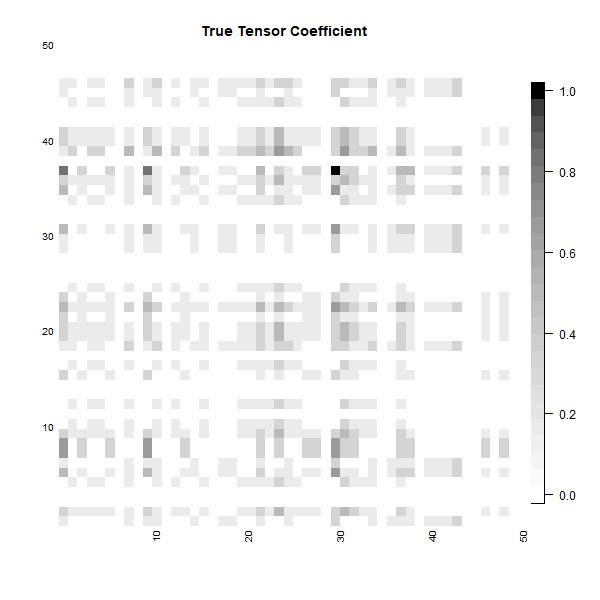
\includegraphics[width=\linewidth]{../Figure/Beta_tens_Scenario1.png}
				\caption{Scene 1}
				\label{fig:scene1}
			\end{minipage}
			\hfill
			\begin{minipage}{0.24\textwidth}
				\centering
				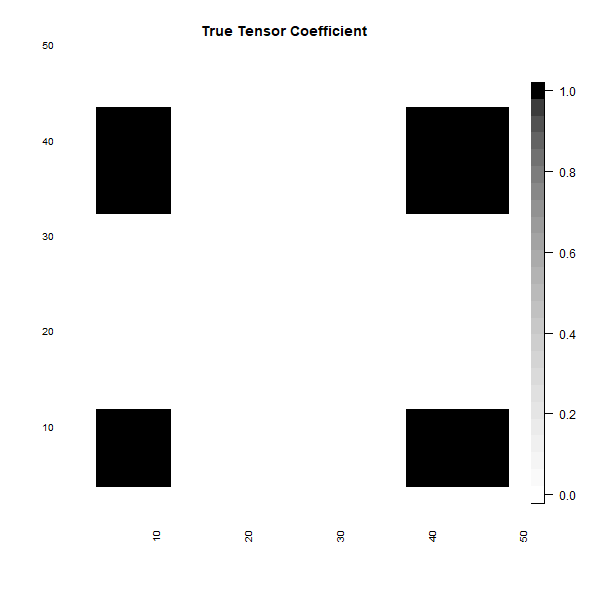
\includegraphics[width=\linewidth]{../Figure/Beta_tens_Scenario2.png}
				\caption{Scene 2}
				\label{fig:scene2}
			\end{minipage}
			\hfill
			\begin{minipage}{0.24\textwidth}
				\centering
				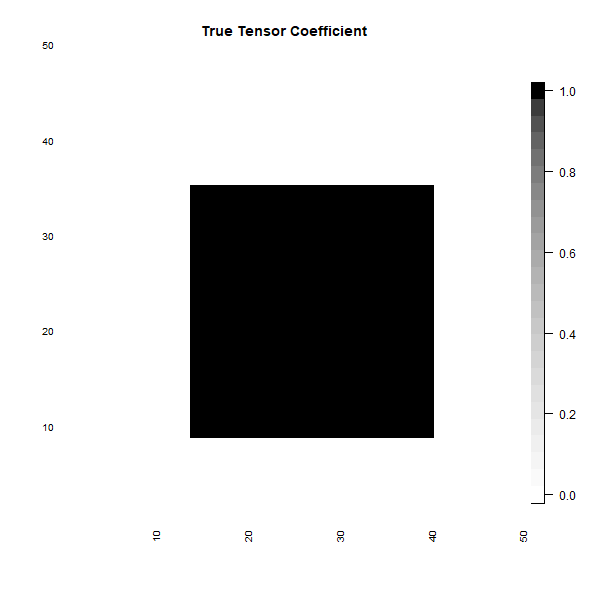
\includegraphics[width=\linewidth]{../Figure/Beta_tens_Scenario3.png}
				\caption{Scene 3}
				\label{fig:scene3}
			\end{minipage}
			\hfill
			\begin{minipage}{0.24\textwidth}
				\centering
				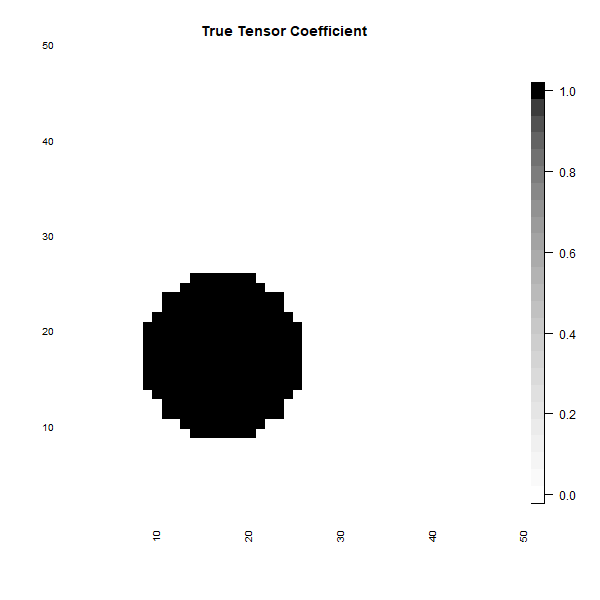
\includegraphics[width=\linewidth]{../Figure/Beta_tens_Scenario4.png}
				\caption{Scene 4}
				\label{fig:scene4}
			\end{minipage}
		\end{figure}
	\end{frame}
	\subsection{模型评估}
	\begin{frame}{模型评估}
		\begin{itemize}[<+->]
			\item 我们使用均方根误差(Root Mean Squared Error, RMSE)与相关系数(correlation coefficient)来评估单元层级张量系数的点估计精度。同时,为了衡量分类准确性,我们计算误分类率(misclassification error)与 F1 分数(F1 score)。
			\item 实验中,我们将数据按 $70{:}30$ 的比例划分为训练集与测试集。用于系数估计与特征选择性能评估的指标在训练集上计算,而分类性能指标在测试集上进行评估。
			\item 为检验新模型的性能,我们选取两种现有的先进分类方法作为对比模型,分别是带有 Lasso 惩罚项的逻辑回归模型(Lasso Logistic Regression)和 L1 范数支持向量机模型(L1-norm Support Vector Machine, SVM).
		\end{itemize}
	\end{frame}
	\begin{frame}{张量数据预测}
		\begin{itemize}[<+->]
			\item 图 \ref{fig:all_scenarios} 展示了使用 BT-SVM 和 BT-LR 估算张量系数的情况。从图中可以看出,我们提出的方法能够广泛地恢复二维张量$\bm{B}$的形状,而不受其形状的影响,也不取决于张量信号是否通过PARAFAC分解构建。
			\item 为了展示预测系数和真实系数之间的相关程度,我们通过图 \ref{fig:residual_maps_all} 展示了不同模型(LR 和 SVM)在不同情景下的表现。
		\end{itemize}
	\end{frame}
	\begin{frame}{张量数据预测}
		\begin{figure}[h]
			\centering
			\begin{minipage}{0.24\textwidth}
				\centering
				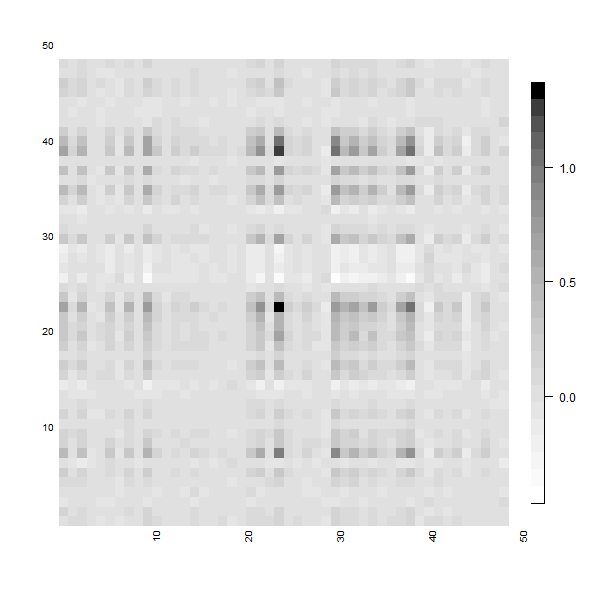
\includegraphics[width=\textwidth]{../Figure/Tensor_estimated_Scenario1_SVM.png}
				\label{fig:scenario1_SVM}
			\end{minipage}
			\hfill
			\begin{minipage}{0.24\textwidth}
				\centering
				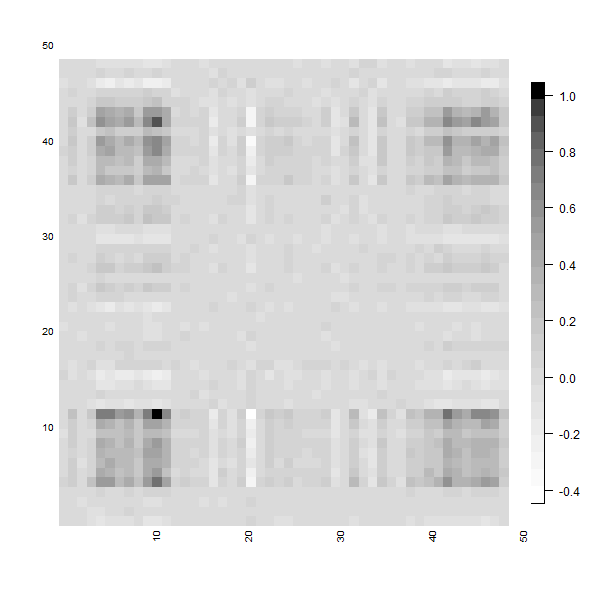
\includegraphics[width=\textwidth]{../Figure/Tensor_estimated_Scenario2_SVM.png}
				\label{fig:scenario2_SVM}
			\end{minipage}
			\hfill
			\begin{minipage}{0.24\textwidth}
				\centering
				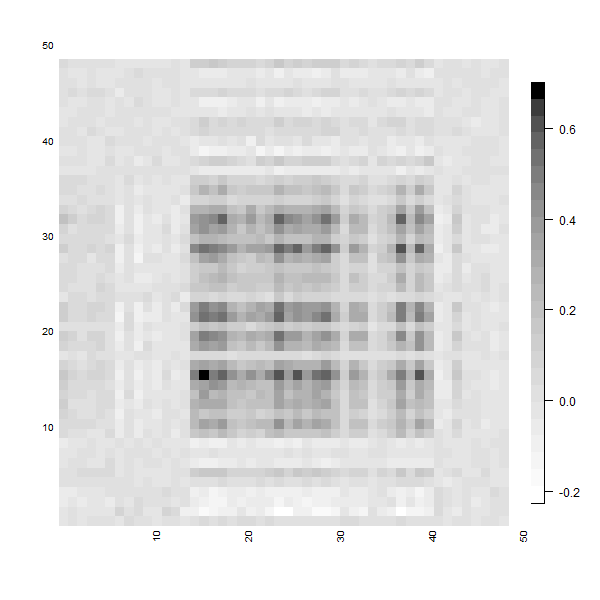
\includegraphics[width=\textwidth]{../Figure/Tensor_estimated_Scenario3_SVM.png}
				\label{fig:scenario3_SVM}
			\end{minipage}
			\hfill
			\begin{minipage}{0.24\textwidth}
				\centering
				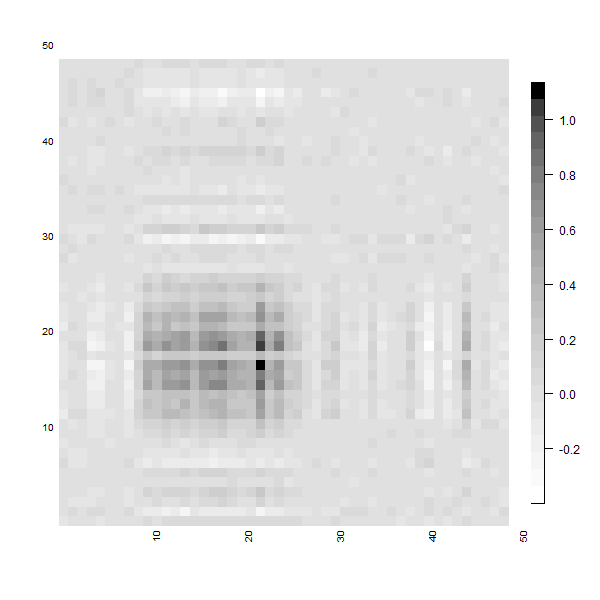
\includegraphics[width=\textwidth]{../Figure/Tensor_estimated_Scenario4_SVM.png}
				\label{fig:scenario4_SVM}
			\end{minipage}
			
			
			\begin{minipage}{0.24\textwidth}
				\centering
				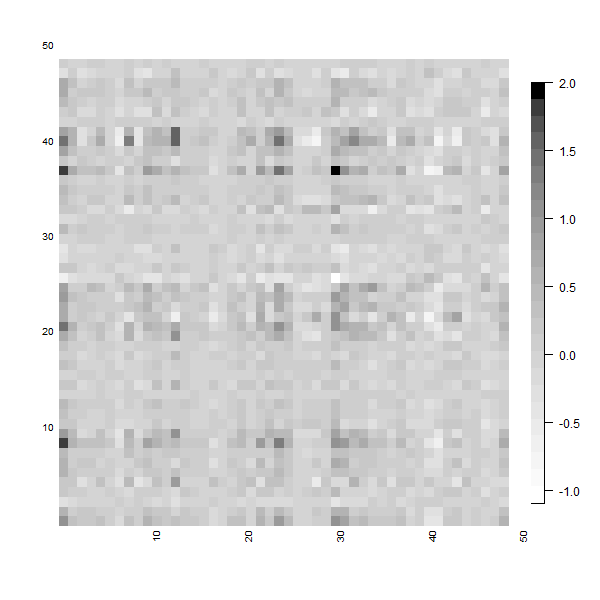
\includegraphics[width=\textwidth]{../Figure/Tensor_estimated_Scenario1_LR.png}
				\label{fig:scenario1_LR}
			\end{minipage}
			\hfill
			\begin{minipage}{0.24\textwidth}
				\centering
				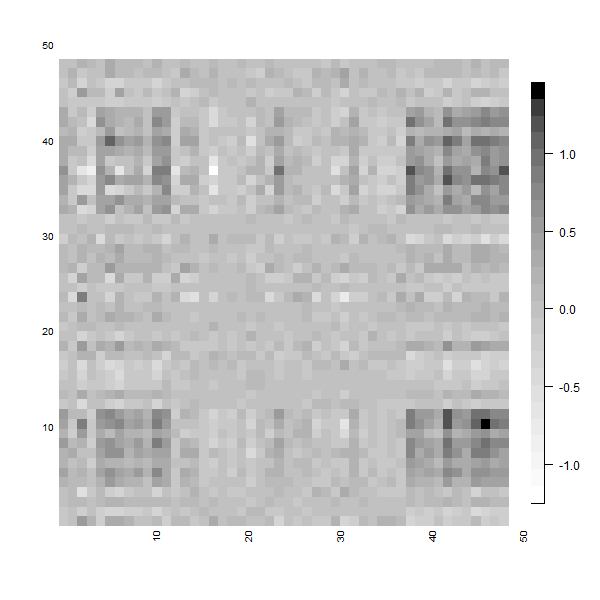
\includegraphics[width=\textwidth]{../Figure/Tensor_estimated_Scenario2_LR.png}
				\label{fig:scenario2_LR}
			\end{minipage}
			\hfill
			\begin{minipage}{0.24\textwidth}
				\centering
				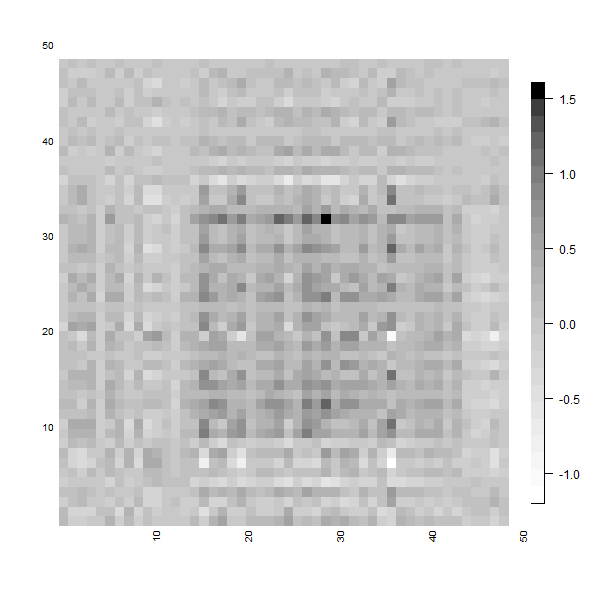
\includegraphics[width=\textwidth]{../Figure/Tensor_estimated_Scenario3_LR.png}
				\label{fig:scenario3_LR}
			\end{minipage}
			\hfill
			\begin{minipage}{0.24\textwidth}
				\centering
				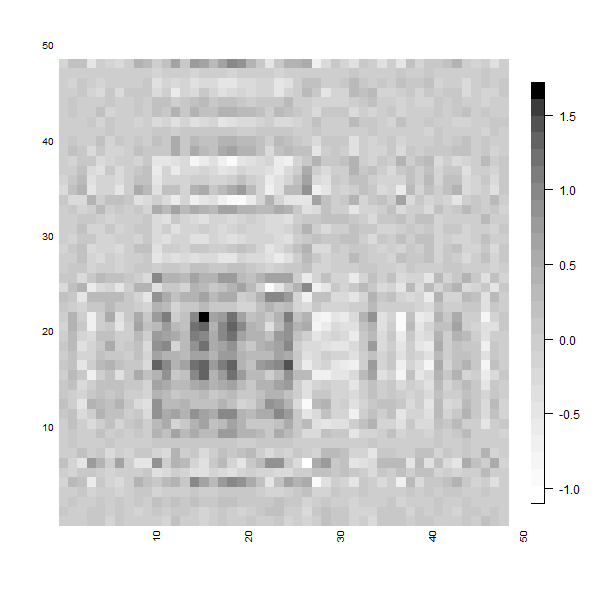
\includegraphics[width=\textwidth]{../Figure/Tensor_estimated_Scenario4_LR.png}
				\label{fig:scenario4_LR}
			\end{minipage}
			
			\caption{估计的张量系数(第一排由BT-SVM模型估计 第二排由BT-LR模型估计)}
			\label{fig:all_scenarios}
		\end{figure}
	\end{frame}
	
	\begin{frame}{残差图}
		\begin{figure}[h]
			\centering
			\begin{minipage}{0.24\textwidth}
				\centering
				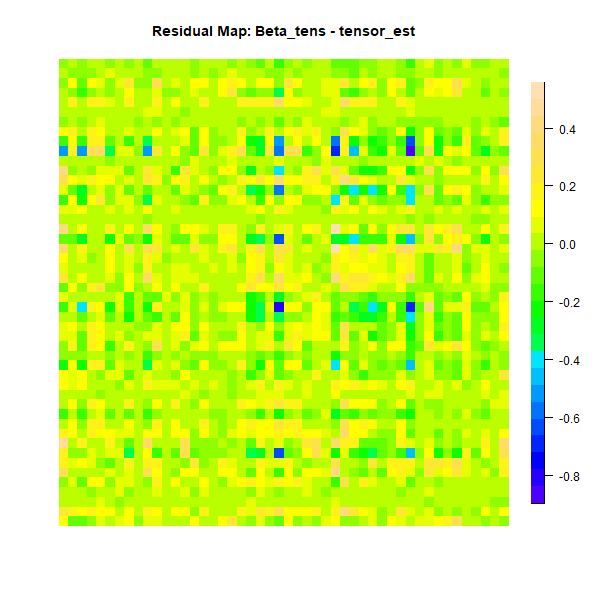
\includegraphics[width=\textwidth]{../Figure/Residual_Tensor_Scenario1_SVM.png}
				\label{fig:residual_scenario1_SVM}
			\end{minipage}
			\hfill
			\begin{minipage}{0.24\textwidth}
				\centering
				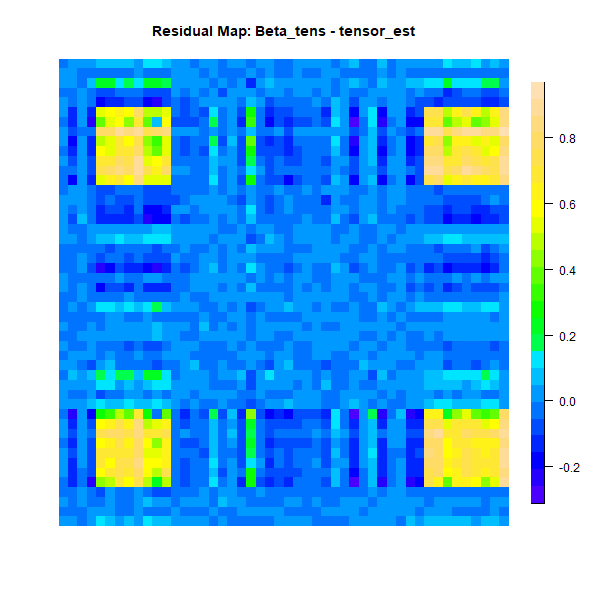
\includegraphics[width=\textwidth]{../Figure/Residual_Tensor_Scenario2_SVM.png}
				\label{fig:residual_scenario2_SVM}
			\end{minipage}
			\hfill
			\begin{minipage}{0.24\textwidth}
				\centering
				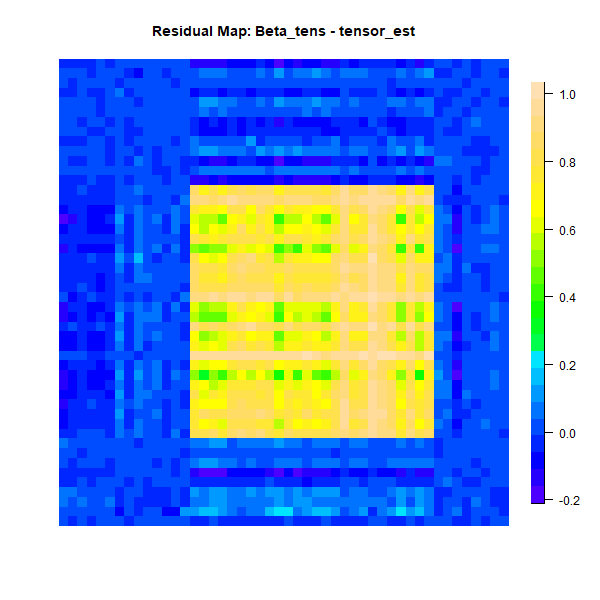
\includegraphics[width=\textwidth]{../Figure/Residual_Tensor_Scenario3_SVM.png}
				\label{fig:residual_scenario3_SVM}
			\end{minipage}
			\hfill
			\begin{minipage}{0.24\textwidth}
				\centering
				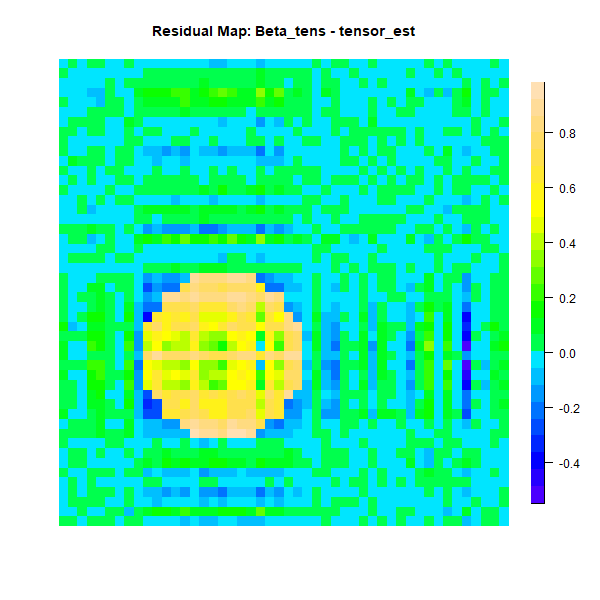
\includegraphics[width=\textwidth]{../Figure/Residual_Tensor_Scenario4_SVM.png}
				\label{fig:residual_scenario4_SVM}
			\end{minipage}
			
			\begin{minipage}{0.24\textwidth}
				\centering
				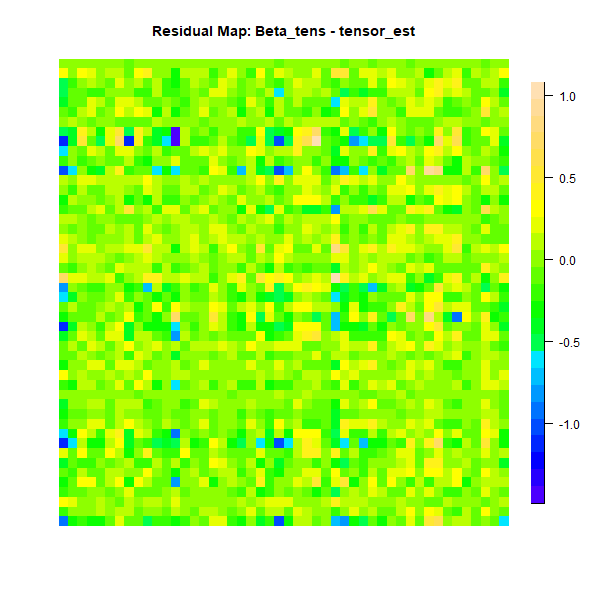
\includegraphics[width=\textwidth]{../Figure/Residual_Tensor_Scenario1_LR.png}
				\label{fig:residual_scenario1_LR}
			\end{minipage}
			\hfill
			\begin{minipage}{0.24\textwidth}
				\centering
				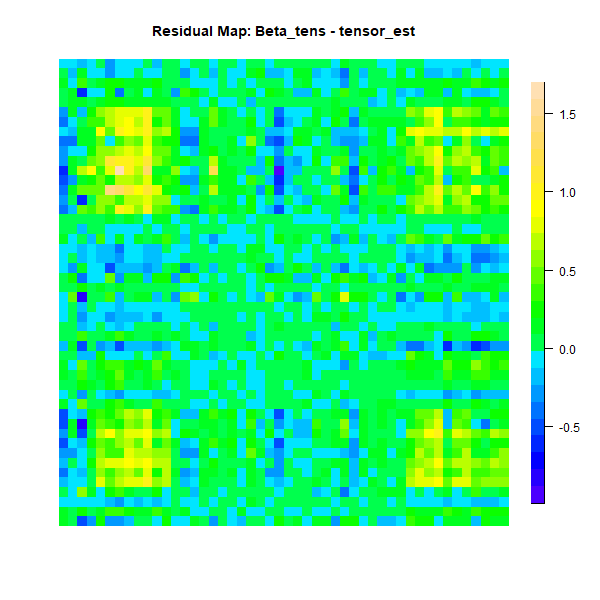
\includegraphics[width=\textwidth]{../Figure/Residual_Tensor_Scenario2_LR.png}
				\label{fig:residual_scenario2_LR}
			\end{minipage}
			\hfill
			\begin{minipage}{0.24\textwidth}
				\centering
				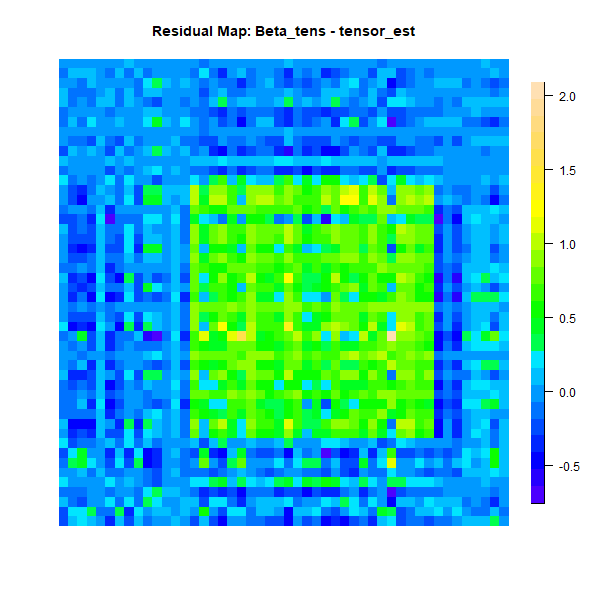
\includegraphics[width=\textwidth]{../Figure/Residual_Tensor_Scenario3_LR.png}
				\label{fig:residual_scenario3_LR}
			\end{minipage}
			\hfill
			\begin{minipage}{0.24\textwidth}
				\centering
				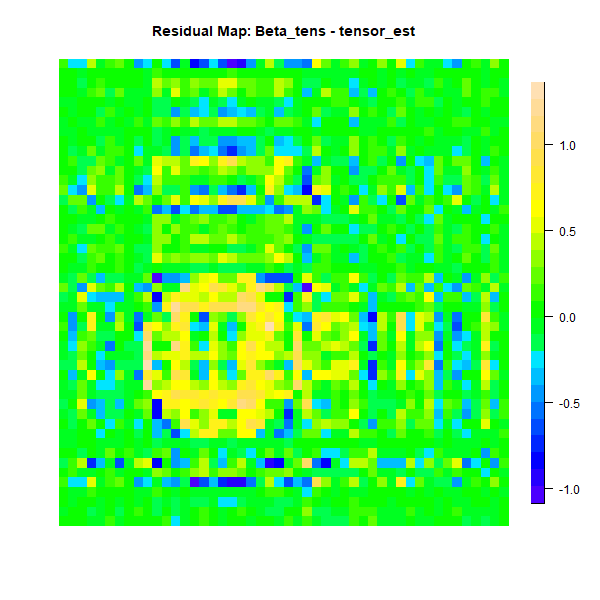
\includegraphics[width=\textwidth]{../Figure/Residual_Tensor_Scenario4_LR.png}
				\label{fig:residual_scenario4_LR}
			\end{minipage}
			
			\caption{残差图}
			\label{fig:residual_maps_all}
		\end{figure}
	\end{frame}
	\begin{frame}{分类性能}
		\begin{itemize}[<+->]
			\item 表 \ref{tab:performance_threeline SVM part1} 和表 \ref{tab:performance_threeline Lasso part1} 中展示了评估模型性能的相关结果,分别对应场景1-4。具体而言,表 \ref{tab:performance_threeline SVM part1} 展示了在二元结果$Y$由SVM Loss生成时的四个场景的结果,而表 \ref{tab:performance_threeline Lasso part1} 则展示了当$Y$来自逻辑损失时的结果。这些结果表明,提出的两种方法(BT-SVM和BT-LR)在系数估计和分类性能上始终优于其他竞争的惩罚方法。
			\item 当二元结果数据来自SVM损失时,BT-SVM方法具有优越的系数估计(如 表\ref{tab:performance_threeline SVM part1} 中较低的 RMSE 和较高的相关系数所示)和改进的分类精度(如表 \ref{tab:performance_threeline SVM part1} 中较低的误分类率和较高的F1分数所示)。即便在数据由逻辑损失生成时,依然有这一特点。
		\end{itemize}
	\end{frame}
	\begin{frame}{分类性能}
		\begin{table}[h!]
			\centering
			\caption{Performance Comparison of Different Methods Across Scenarios; Y generated from SVM Loss.}
			\label{tab:performance_threeline SVM part1}
			\resizebox{\textwidth}{!}{ % 调整表格宽度到页面宽度
				\begin{tabular}{llcccc}
					\toprule 
					\textbf{Scenarios} & \textbf{Methods} & \textbf{RMSE} & \textbf{Corr.Coef.} & \textbf{Mis. Class.} & \textbf{F1-score} \\
					\midrule
					\multirow{4}{*}{Scenario 1} & LR w/ lasso & 0.186 & 0.118 & 0.500 & 0.576 \\
					& L1norm-SVM & 0.129 & 0.233 & 0.413 & 0.523 \\
					& BT-SVM & 0.127 & 0.591 & 0.340 & 0.653 \\
					& BT-LR & 0.197 & 0.449 & 0.360 & 0.640 \\
					\midrule
					\multirow{4}{*}{Scenario 2} & LR w/ Lasso & 0.395 & 0.057 & 0.520 & 0.487 \\
					& L1norm-SVM & 0.393 & 0.168 & 0.433 & 0.591 \\
					& BT-SVM & 0.285 & 0.820 & 0.193 & 0.803 \\
					& BT-LR & 0.330 & 0.505 & 0.347 & 0.653 \\
					\bottomrule
				\end{tabular}
			}
		\end{table}
	\end{frame}
	
	\begin{frame}{分类性能}
		\begin{table}[h!]
			\centering
			\caption{Performance Comparison of Different Methods Across Scenarios; Y generated from SVM Loss.}
			\label{tab:performance_threeline SVM part2}
			\resizebox{\textwidth}{!}{ % 调整表格宽度到页面宽度
				\begin{tabular}{llcccc}
					\toprule 
					\textbf{Scenarios} & \textbf{Methods} & \textbf{RMSE} & \textbf{Corr.Coef.} & \textbf{Mis. Class.} & \textbf{F1-score} \\
					\midrule
					\multirow{4}{*}{Scenario 3} & LR w/ Lasso & 0.541 & 0.064 & 0.453 & 0.585 \\
					& L1norm-SVM & 0.539 & 0.166 & 0.407 & 0.639 \\
					& BT-SVM & 0.430 & 0.768 & 0.227 & 0.788 \\
					& BT-LR & 0.454 & 0.570 & 0.320 & 0.684 \\
					\midrule
					\multirow{4}{*}{Scenario 4} & LR w/ Lasso & 0.315 & 0.178 & 0.407 & 0.639 \\
					& L1norm-SVM & 0.315 & 0.213 & 0.440 & 0.554 \\
					& BT-SVM & 0.221 & 0.769 & 0.207 & 0.805 \\
					& BT-LR & 0.276 & 0.529 & 0.347 & 0.679 \\
					\bottomrule
				\end{tabular}
			}
		\end{table}
	\end{frame}
	
	\begin{frame}{分类性能}
		\begin{table}[h!]
			\centering
			\caption{Performance Comparison of Different Methods Across Scenarios; Y generated from Lasso Loss.}
			\label{tab:performance_threeline Lasso part1}
			\resizebox{\textwidth}{!}{ % 调整表格宽度到页面宽度
				\begin{tabular}{llcccc}
					\toprule
					\textbf{Scenarios} & \textbf{Methods} & \textbf{RMSE} & \textbf{Corr.Coef.} & \textbf{Mis. Class.} & \textbf{F1-score} \\
					\midrule
					\multirow{4}{*}{Scenario 1} & LR w/ lasso & 0.175 & 0.078 & 0.493 & 0.580 \\
					& L1norm-SVM & 0.192 & 0.208 & 0.527 & 0.448 \\
					& BT-SVM & 0.120 & 0.701 & 0.220 & 0.793 \\
					& BT-LR & 0.230 &  0.456 & 0.340 & 0.698 \\
					\midrule
					\multirow{4}{*}{Scenario 2} & LR w/ Lasso & 0.395 & 0.128 & 0.547 & 0.474 \\
					& L1norm-SVM & 0.393 & 0.215 & 0.453 & 0.534 \\
					& BT-SVM & 0.233 & 0.880 & 0.140 & 0.844 \\
					& BT-LR & 0.284 & 0.670 & 0.233 & 0.788 \\
					\bottomrule
				\end{tabular}
			}
		\end{table}
	\end{frame}
	
	\begin{frame}{分类性能}
		\begin{table}[h!]
			\centering
			\caption{Performance Comparison of Different Methods Across Scenarios; Y generated from Lasso Loss.}
			\label{tab:performance_threeline Lasso part2}
			\resizebox{\textwidth}{!}{ % 调整表格宽度到页面宽度
				\begin{tabular}{llcccc}
					\toprule
					\textbf{Scenarios} & \textbf{Methods} & \textbf{RMSE} & \textbf{Corr.Coef.} & \textbf{Mis. Class.} & \textbf{F1-score} \\
					\midrule
					\multirow{4}{*}{Scenario 3} & LR w/ Lasso & 0.542 & 0.050 & 0.427 & 0.467 \\
					& L1norm-SVM & 0.539 & 0.149 & 0.413 & 0.544 \\
					& BT-SVM & 0.426 & 0.811 & 0.187 & 0.823 \\
					& BT-LR & 0.414 & 0.555 & 0.313 & 0.647 \\
					\midrule
					\multirow{4}{*}{Scenario 4} & LR w/ Lasso & 0.316 & 0.127 & 0.447 & 0.518 \\
					& L1norm-SVM & 0.315 & 0.193 & 0.473 & 0.530 \\
					& BT-SVM & 0.221 & 0.739 & 0.213 & 0.790 \\
					& BT-LR & 0.317 & 0.479 & 0.360 & 0.635 \\
					\bottomrule
				\end{tabular}
			}
		\end{table}
	\end{frame}
	\subsection{MRI脑肿瘤分类}
	
	\begin{frame}{脑肿瘤MRI图像分类}
		\begin{itemize}
			\item 数据集包含155张脑部肿瘤切片MRI图像和98张正常MRI图像。我们对比了 BT-SVM ,BT-LR,带Lasso惩罚的逻辑回归以及L1norm-SVM对该数据集的分类性能。 
			测试结果见表 \ref{tab:performance_threeline MRI}。
			\begin{table}[h]
				\centering
				\caption{不同模型的分类性能}
				\label{tab:performance_threeline MRI}
				\begin{tabular}{llcccc}
					\toprule
					\textbf{Methods} & \textbf{Mis. Class.} & \textbf{F1-score} \\
					\midrule
					LR w/ lasso & 0.333 & 0.702  \\
					L1norm-SVM & 0.451 & 0.709 \\
					BT-SVM & 0.211 & 0.855 \\
					BT-LR & 0.303 &  0.763  \\
					\bottomrule
				\end{tabular}
			\end{table}
		\end{itemize}
	\end{frame}
	\section{参考文献}
	
	\begin{frame}[allowframebreaks]
		\begin{thebibliography}{99}
			\bibitem{a}Bi X, Tang X, Yuan Y, et al. Tensors in statistics. \textit{Annual Review of Statistics and Its Application}, 2021, 8(1): 345–368.
			\bibitem{b}Tucker L R. Some mathematical notes on three-mode factor analysis[J]. \textit{Psychometrika}, 1966, 31(3): 279-311.
			\bibitem{c}Polson N G, Scott S L. Data augmentation for support vector machines[J]. 2011.
			\bibitem{d}Polson N G, Scott J G, Windle J. Bayesian inference for logistic models using Pólya–Gamma latent variables. \textit{Journal of the American Statistical Association}, 2013, 108(504): 1339–1349.
			\bibitem{e}Guhaniyogi R, Qamar S, Dunson D B. Bayesian tensor regression[J]. \textit{Journal of Machine Learning Research}, 2017, 18(79): 1-31.
		\end{thebibliography}
	\end{frame}
	
	\begin{frame}
		\begin{center}
			{\Huge\calligra Thanks!}
		\end{center}
	\end{frame}
	
\end{document}